\documentclass{article}

\usepackage{graphicx}
\usepackage[shortlabels]{enumitem}


\newcommand{\twopartdef}[4]
{
    \left\{
    \begin{array}{ll}
        #1 & #2 \\
        #3 & #4
    \end{array}
    \right.
}

\newcommand{\threepartdef}[6]
{
    \left\{
    \begin{array}{ll}
        #1 & #2 \\
        #3 & #4 \\
        #5 & #6
    \end{array}
    \right.
}

\begin{document}

\title{Time Range Queries for Hereditary Properties \\ \large 6.854 Final Project}
\author{Arsen Mamikonyan, Hayk Saribekyan}

\maketitle

\begin{abstract}
    Time range queries are important for analysing large datasets with timestamps. Such datasets are common in computational geometry, where a sequence of points with timestamps often corresponds to a trajectory of an object. Time range queries in this case check a certain property of section of the trajectory.
    
    In this paper we review recent general frameworks that can be used to handle property testing queries for time ranges, and discuss their implementations for solving certain problems in computational geometry. The results are limited to \textit{hereditary} properties, which cover a large variety of interesting problems.
    
    For two different hereditary properties, we compared the performance of efficient an algorithm and a naive one in practice. We observed that the efficient algorithms require more than ten times the amount of code in certain cases, but the large constant factor associated with it is compensated when working with large datasets.
\end{abstract}

\section{Introduction}
\label{sec:intro}

TODO: add normal references (maybe to envelopes), see the first paper, where in the first page there are a lot of motivational references.

With the abundance of GPS and other movement tracking sensors there is a large amount of timestamped location data. The movement of an object in space can be modelled by a sequence of points $S = s_1, \dots, s_n$. To analyse the trajectory of the movement, one may want to check a certain property $P$ for portions $S[i, j] = s_i, \dots, s_j$ of $S$ for given values of $i$ and $j$. This paper discusses how to efficiently address such queries when $P$ satisfies the following two properties:
\begin{itemize}
    \item $P$ is boolean.
    \item $P$ is hereditary. This means that for a given sequence $S$, if $P(S)$ is true, then $P(S')$ is true for any continuous subsequence $S'$ of $S$.
\end{itemize}

In this paper we discuss and implement two properties for a sequence of points $S = s_1, \dots, s_n$:
\begin{itemize}
    \item \textit{Monotonicity}:  $S$ is \textit{monotone} if there is a direction vector $v$ such that TODO. In terms of trajectories, monotonicity shows whether the object travelled more or less in the same direction.
    
    \item \textit{Closeness}: $S$ is \textit{close} if any pair of points in $S$ is at most of distance $1$. One could use closeness queries to detect if a moving object mostly stayed in the same surrounding.
\end{itemize}

For a property $P$ satisfying the restrictions above, let $j^*(i)$ be the largest index $j$ such that $P$ holds for $S[i, j^*(i)] = s_i, \dots, s_{j^*(i)}$. Now notice, that since $P$ is a hereditary property $P(S[i, j]) = true$ if and only if $i \leq j \leq j^*(i)$. Therefore, if we construct $j^*(i)$ we can answer property testing queries in $O(1)$. Therefore, for the rest of the paper our goal will be to efficiently compute $j^*(i)$.

Bokal et al. \cite{bokal2015} propose an algorithms that compute $j^*(i)$ in $O(n)$ time for monotonicity, and in $O(n\log^2 n)$ time for closeness. Chan and Pratt \cite{chan2016} describe a different algorithm to achieve the same result for closeness, but also improve it to $O(n\log n)$ using fractional cascading.

The rest of the paper is organized as follows: Section \ref{sec:naive}
describes the naive algorithms we developed to solve the problems
we selected; in Section \ref{sec:monotonicity} we review the general
framework that is set in \cite{bokal2015} for solving time range
query problems, and show how it is applied to compute $j^*(i)$ for
monotonicity. Section \ref{sec:closeness} reviews the framework by
\cite{chan2016} and its application for the closeness property. We
then give some implementation details in Section \ref{sec:implementation},
and describe the experimental setup and our tests in Section
\ref{sec:experiments}.

\section{Naive Algorithms}
\label{sec:naive}
Suppose that for a sequence of length $n$ a property $P$ can be checked in $T_P(n)$ time. Then, one can compute $j^*(i)$ using binary search for each $i$. On a step of a binary search concerning a range $[l, r]$ the algorithm would spend $T_P(r - l)$ time. The total runtime of this simple algorithm is $O(nT_P(n)\log n)$. Call this algorithm $SN$ (stands for super-naive). For the problems of monotonicity and closeness we can do better.

\subsection{Monotonicity}
\label{sec:naive:monotonicity}
To detect whether a sequence is monotone or no, we can process the points while keeping a set of polar angles (field-of-view or FoV) that a direction vector $v$ can have. Notice that the FoV is always an interval. When a new point arrives we can update the FoV in constant time. If the FoV ever becomes empty, then the given sequence is not monotone. This algorithm runs in $O(n)$ time for a sequence of length $n$. Using this submodule for $SN$ we would get a $O(n^2\log n)$ algorithm for computing $j^*(i)$ for all values of $i$.

However, doing a binary search for monotonicity is redundant, since we will do the same computation many times. Instead, for each $i$ proceed with the FoV computation until it is empty, which will happen precisely when we reach $j^*(i) + 1$. The resulting algorithm runs in $O(n^2)$ time.

\subsection{Closeness}
\label{sec:naive:closeness}
The simple method of closeness-check takes $O(n^2)$ for a sequence of $n$ points, because one has to check all pairs of points. This results in $SN$ runtime of $O(n^3\log n)$, which is super-slow. We can improve the closeness-check to $O(n\log n)$ using furthest-point Voronoi diagrams, but that would not qualify for $SN$ and would also take $O(n^2 \log^2 n)$ time to compute, which is also not fast.

Define $k^*(i)$ as the largest index such that $d(s_i, s_j) \leq
1$ for all $j \leq k^*(i)$. Clearly, $k^*(i) \geq j^*(i)$ because we are checking for a weaker property. Also,
notice that $k^*$ can be computed in $O(n^2)$ for all points by calculating all pairwise distances.

Noticing that 
\begin{equation}
\label{kj_rel}
j^*(i) = \min( j^*(i + 1), k^*(i) )
\end{equation}
, we can calculate
$j^*(i)$ for all points in $O(n)$ extra time if we are given all
values for $k^*(i)$. So we found a $O(n^2)$ algorithm for computing
closeness property for all subsequences.

\section{Monotonicity in Linear Time}
\label{sec:monotonicity}
Bokal et al. introduced an elegant framework to deal with range queries for hereditary problems. The key idea in their work is to greedily split the given set of points into ranges, defined by anchor points, and solve for each using a divide and conquer. To simplify the reasoning we first define a property matrix $A_P$ such that
\[ A_P(i, j) = \twopartdef{1}{P(S[i, j]) = true}{0}{P(S[i, j]) = false} \]

See Figure \ref{fig:property_matrix} for an example. Suppose that
there is an algorithm $J_P$ that, for a given $i$, finds $j^*(i)$
(notice that even if such $J_P$ exists, we are not happy to run it
$n$ times for each $i$). We use $J_P$ to find \textit{anchor} points
in $S$ as follows. Let $a_k$ be the index of $k^{th}$ anchor point
in $S$. We define $a_1 = s_1$, $a_k = \max(1 + a_{k-1}; j^*(a_{k-1}))$
for $k > 1$. Thus, the anchor points can be found using $J_P$.
Figure \ref{fig:property_matrix} shows the anchor points on $A$
(leftmost image).

\begin{figure}
    \centering
    \makebox[\textwidth][c]{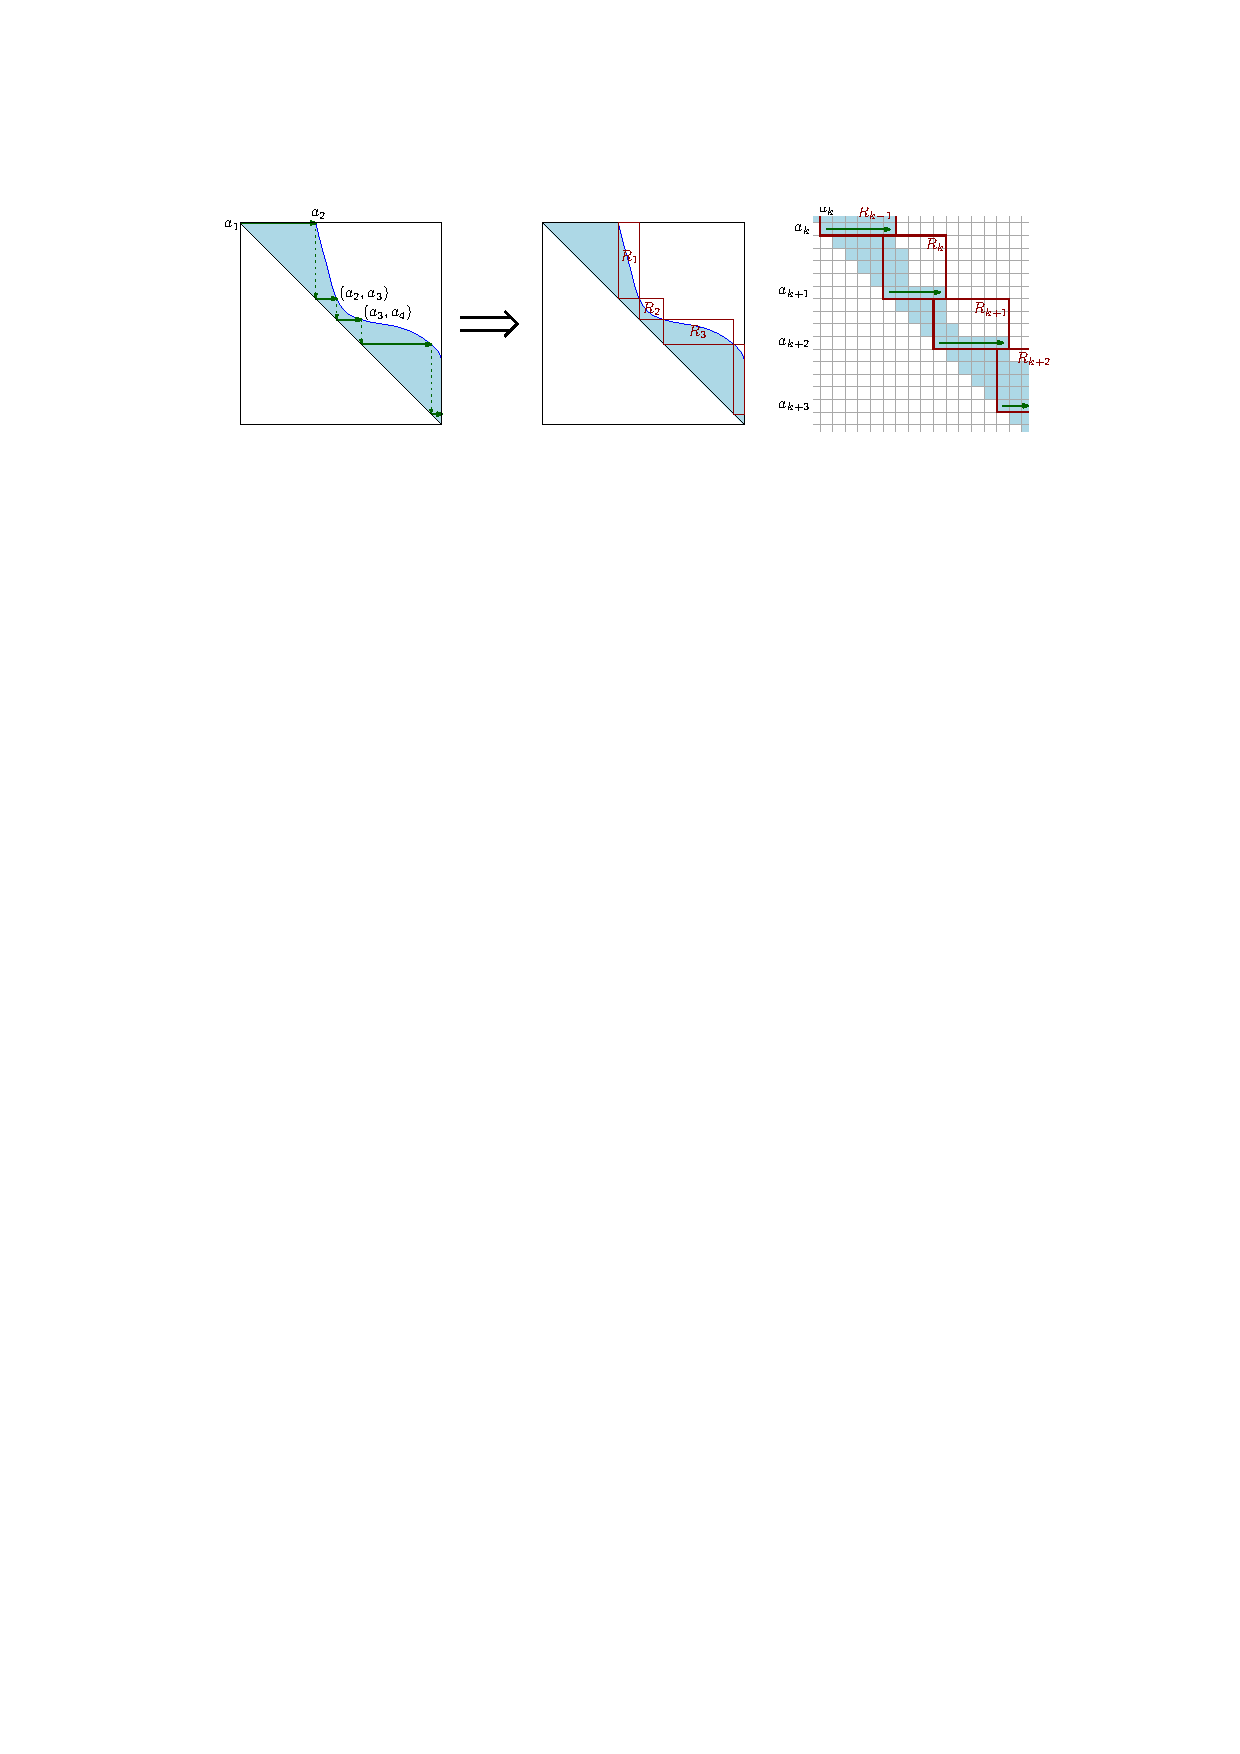
\includegraphics[width=1.1\textwidth]{figures/property_matrix.pdf}}
    \label{fig:property_matrix}
    \caption{The property matrix $A_P$. The blue regions show the locations that are 1. The left image illustrates the anchor points. The middle one shows the greedily constructed rectangles from the anchor points. On the right side is the detailed view of the property matrix. Figure from \cite{bokal2015}.}
\end{figure}

Also shown in Figure \ref{fig:property_matrix} are rectangles formed using the anchor points. If we solve a rectangle (find the curve in $A$ separating 1's from 0's) for each rectangle, then we will be done, as stated in Lemma 2.1 from Bokal et al.

\textbf{Lemma 2.1} Assume that we have the following two subroutines for sequence $S$ and a property $P$:
\begin{enumerate}[(a)]
    \item For any $a = 1, \dots, n$ find the $j^*(a)$, taking $T_{greedy}(j^*(a) - a)$
    \item Solve a rectangle with anchor points at opposite vertices (anchored rectangles). Suppose this module takes $T_{rect}(height(R) + width(R))$.
\end{enumerate}

Both of these modules are property specific, but Bokal et al. make another interesting generic step that explains how solving rectangles can be done using a divide-and-conquer approach. We will, however, skip that step and focus on the problem of monotonicity. It turns out that monotonicity does not require the divide-and-conquer approach to solve anchored rectangles.

\subsection{Solving Monotonicity}
Section \ref{sec:naive:monotonicity} discusses how to find $j^*(i)$ in linear time for a given $i$ by using intervals of polar angles. This algorithm will serve as the subroutine for Lemma 2.1(a).

Consider an anchored rectangle $R$ with a lower-left corner $(a, a)$, width $w$ and height $h$.
\begin{enumerate}[-]
\item By traversing the points $S[a, a + w]$, we can compute for each $j = a, \dots, a + w$ the interval of polar angles $I_j$ such that $S[a, j]$ is monotone with respect to all directions in $I_j$.
\item By traversing the points $S[a - h, a]$ in reverse order, a similar set $I_i$ can be computed for $a - h \leq i < a$, representing the set of monotone directions for $S[i, a]$.
\end{enumerate}

If $i < a < j$, then $S[i, j]$ is monotone if and only
if $I_i$ and $I_j$ have a non-empty intersection. Thus, for each
$i = a - h, \dots, a$, $j^*(i)$ is the largest index such that $I_i
\cap I_{j^*(i)} \neq \emptyset$.
Noting that search for $j^*(i+1)$
can start from $j^*(i)$, we can compute $j^*(i)$ for all $i \in [a
- h, a]$ in linear time.

These two subroutines, together with Lemma 2.1 give a linear solution
to the monotonicity problems. We have evaluated Naive algorithm
(from Section \ref{sec:naive}) and this algorithm in Section
\ref{sec:experiments}.

%This is where divide and conquer strategy is used. Consider a rectangle $R$ with rows $[a, a + h]$ and columns $[b, b + w]$. We can set $m = a + [h / 2]$ and using $J_P$ find $j^*(m)$. If $m \leq i \leq a + h$ then $j^*(i) \geq j^*(m)$, and if $a \leq i \leq m$ then $j^*(i) \leq j^*(m)$. Therefore, once we know the value of $j^*(m)$ the solution for $R$ can be computed using two recursive calls to its upper-left and lower-right sub-rectangles.

%Notice, however, this type of recursion will just end up calling $J_P$ for all indices in $[a, a + h]$, having no divide-and-conquer effect.

\section{Closeness in $O(n \log^2 n)$}
\label{sec:closeness}

Chan, Prat \cite{chan2016} take a different approach to calculating
hereditary properties, they first efficiently calculate $k^*$ values
for all the pairs using a range tree \cite{lueker1978data} that has a secondary structure
to make querying faster, and then they calculate $j^*$ values from
those.

During the first part of the algorithm we want a data structure
that given a point $i$, could efficiently answer what is the point
with smallest index $k^*(i)+1$ that lies outside a unit circle
centered at $i$. To do this without running a binary search we build
the following range tree.

\begin{figure}
    \centering
    \makebox[\textwidth][c]{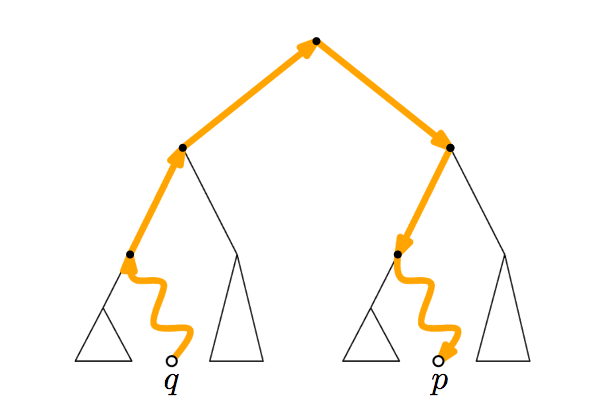
\includegraphics[width=0.5\textwidth]{figures/query_path}}
    \label{fig:query_path}
    \caption{A search path finding $p = k^*(q) + 1$ of point $q$.
    The search goes up until it find a range where $p$ lies and
    then goes down narrowing down the range until it reaches the
    leaf $p$.
    Figure from \cite{chan2016}.}
\end{figure}

First we build a regular 1 dimensional range tree using indices of
the data points. In order to answer queries efficiently, at each
node $v$ we store intersections of circles centered at points
belonging to the range of that node $v$. Once we have this tree
that can answer query at each node in $Q(v)$ time, notice that the
following algorithm will give us $O(Q(v) \log n)$ time algorithm for
finding $k^*(i)$ for a single point.

Algorithm will starts at query point $q$ (see Figure \ref{fig:query_path})
\begin{enumerate}[-]
\item
In the first ``up'' phase, we walk upward from $q$ towards the root.
Each time we go up from a left child, we query the secondary structure
at righ sibling, to see if there exists a point in that range that
is far from $q$.
\begin{itemize}
\item If no, we can extend the search by going one more level up.
\item If yes, the first point far from $q$ is in the right child, so we proceed to the second step to locate that node.
\end{itemize}


\item In the second (``down'') phase, we walk downward from the
current node to a leaf to locate the far point with smallest index. Each time we descend from a node,
we query the secondary structure at the left child to see if there exists a point in the left child's range that is far from $q$
\begin{itemize}
\item If no, the point that's far from $q$ lies in the range of the right child, so we descend right.
\item If yes, we descend left.
\end{itemize}
\end{enumerate}


After we find $k^*(i)$ for all the nodes, we combine those using
Equation \ref{kj_rel} in $O(n)$ time. Which gives total runtime of
$O(n \log n Q(n))$. Now we present the seqondary data structure
that has query time $Q(n) = \log n$, and total build time $O(n \log
n)$

Using sweep line \cite{shamos1976geometric} technique (more in Section \ref{sec:implementation})
we can merge two intersections of circles in linear time. This is
possible because intersections of circles is very similar to a
convex hull, but instead of a polygon it has arcs connecting vertices
instead of line segments. We call this data structe a \textit{polyarc}.

By adding \textit{polyarc}s to nodes of the range tree (based on indices)
from bottom to up, at each level we'll spend $O(n)$ time since the
merging of \textit{polyarc}s is done in linear time, so total construction
time will be $O(n \log n)$, and we can answer contins queries in
$O(\log (n))$ time by doing binary search to which arc the query
point $q$ might belong using the $x$ coordinate of $q$ and $x$
coordinates of the vertices of the \textit{polyarc}.

\section{Implementation Details}
\label{sec:implementation}
In the papers reviewed here (\cite{bokal2015,chan2016}) there are at least 6 algorithms presented. We wanted to implement algorithm that use frameworks of both papers. In order to limit the size of the implementation we decided to pick monotonicity property for its simplicity (and elegance), which was solved in Bokal et al. \cite{bokal2015}. We chose to implement the closeness testing algorithm from \cite{chan2016} because it used many ideas from the class, for example the intersection of convex envelopes in 2 dimensions, range trees.

The implementations of naive algorithms as well as of the efficient monotonicity testing algorithm are relatively easy, so in this paper we skip discussing them. We implemented the $O(n \log ^2 n)$ algorithm for solving closeness testing from \cite{chan2016}.  The algorithm has two distinct parts: a high-level tree-range data structure, and a lower-level data structure for storing \textit{polyarcs} (see Section \ref{sec:closeness}).
Higher level algorithm was easier of the two, it involved implementing a range tree and the querying algorithm described in Section \ref{sec:closeness}.

A polyarc is a convex geometric shape, which is defined by a clockwise set of its vertices like a polygon. Unlike a polygon, each edge of a polyarc is an arc of a circle. The algorithm needs to be able to find the intersection of two polyarcs, and also decide whether a query point is inside the polyarc.

Both of these algorithms are similar to those of polygons, but the majority of the implementation effort was spent to handle the cases specific to polyarcs. Our representation of polyarcs has two ``sides'': upper and lower, respectively the upper part of the complex shape and the lower one. To intersect two polyarcs we first found a minimal upper envelope i.e. for each $x$ coordinate found recorded the polyarc, which had a lower upper side. Similarly, we computed a maximal lower envelope. The area above the maximal lower envelope and minimal upper envelope is the intersection of two polyarcs. Each of these steps can be performed in linear time by a sweep line technique.

The envelope representation of polyarcs is also helpful for querying whether a point is inside the polyarc or no. One needs to simply do a binary search for the $x$ coordinate of the candidate point.
If a vertical line at that location crosses the higher envelope on a larger value of $y$ than the lower envelope, then the query point is inside the polyarc.

Overall, we wrote more than 1200 lines of code in C++ for the implementation of the algorithms, and 800 lines of code for testing. Large part of the code is dedicated to the closeness algorithm in $O(n \log^2 n)$. We used C++ for the implementation so that the overhead that the language adds to the runtime is minimized. A simple language to write code in is Python, but we think that in this case the strong type checking of C++ helped us, because of a complex structure of the code. 

\section{Experimental Results}
\label{sec:experiments}
We have tested the performance of the algorithms we've implemented with synthetic datasets, that we have tried to model based on some potential problems where the algorithms could have been used.
% - mention that we have used random walk to mimic reality. in that case the good algorithm for monotonicity is not that good. but for the worst case, it's great.
% - 

\subsection{Monotonicity}

\begin{figure}[!ht]
  \centering
  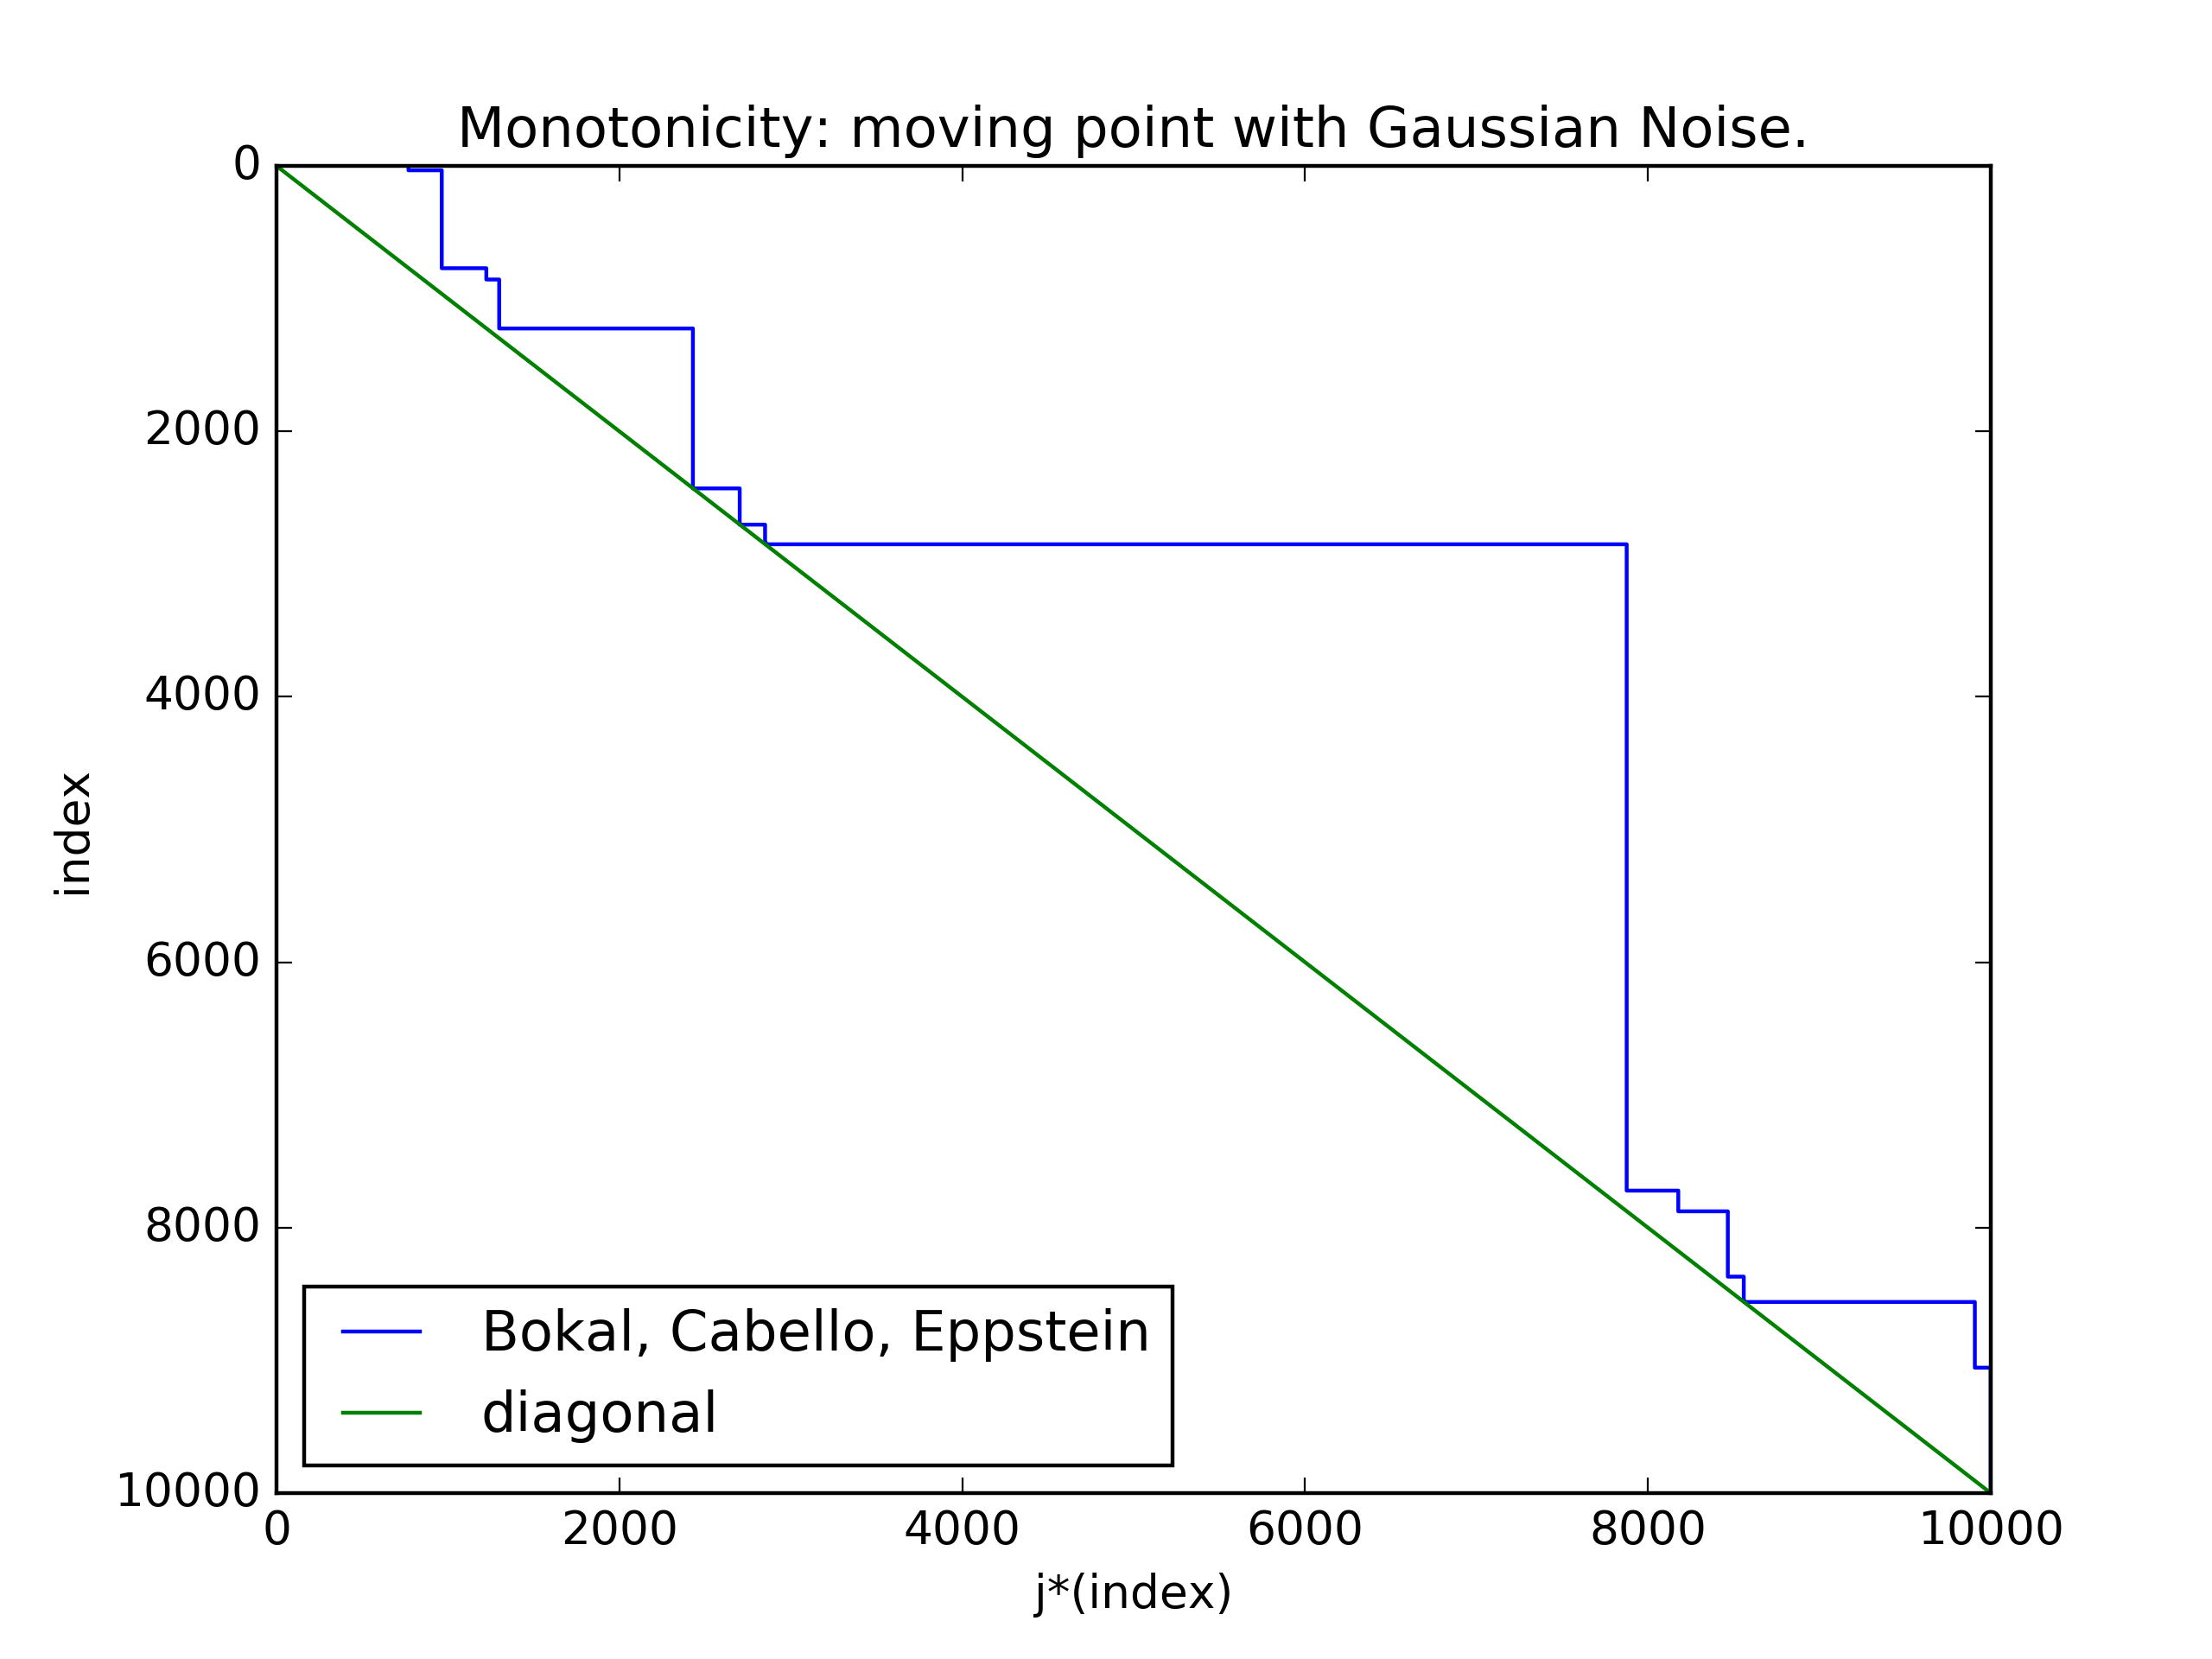
\includegraphics[height=8cm]{../plots/monotonicity_moving_gaussian}
  \caption{Property matrix for movement monotonicity for time intervals for a point moving steadily in $x$ direction with Gaussian noise with $\sigma_x = 0.05, \sigma_y = 1$.}
  \label{fig:monotonicity_demo}
\end{figure}

For monotonicity we have tried looking at a tajectory of a particle
moving steadily along $x$ axis, but with some noise added to the
movement. And the goal is to find all subsequences of intervals
that the trajectory had some constant direction. In Figure
\ref{fig:monotonicity_demo} you can see the property matrix (i.e. the region where the property holds) when the noise added is a Gaussian
noise with standard deviations $\sigma_x = 0.05, \sigma_y = 1$.

You can see that the area of the region where the property is substential, so we expect Naive algorithm to perform worse than the faster version that we've implemented. 
Figure \ref{fig:monotonicity_comparison} shows runtime differences in millliseonds between Naive algorithm and algorithm we presented from Bokal et al.

TODO: Informative plot for gaussian... Actually make plots double plots (side by side, for 2 examples we are going to show) TODO TODO

Whereas if we look at a different dataset, e.g. a random walk, the
performance results could be different. Figure
\ref{fig:monotonicity_random_walk} shows the property matrix for a
random walk, and Figure \ref{fig:monotonicity_comparison_2} shows
that the runtimes of the two algorithms are actually very close in
practice for this case.

\begin{figure}[!ht]
  \centering
  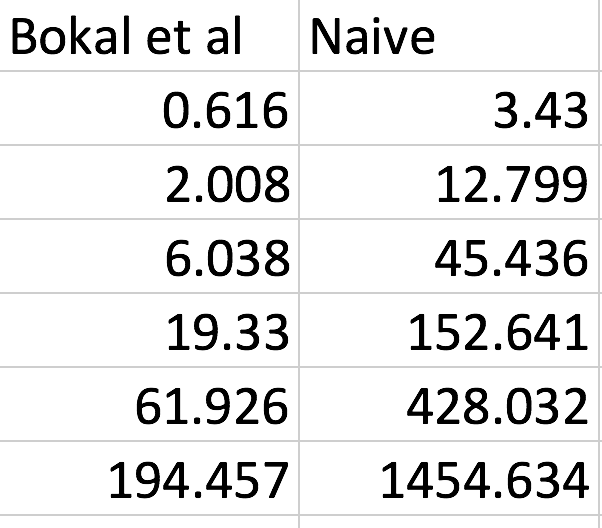
\includegraphics[height=5cm]{figures/monotonicity_comparison}
  \caption{Runtimes (in millseconds) of Naive and Bokal et. al}
  \label{fig:monotonicity_comparison}
\end{figure}

\subsection{Closeness}

For testing the closeness algorithm, we have generated points from a random walk.
At each step we uniform randomly pick a direction, and move 0.3
distance in that direction. And we want to know all subsequences
of the walk that are clustered together within distance of 1.

Figure \ref{fig:diameter_demo} shows the property matrix when running
closeness algorithm on the random walk data, and
\ref{fig:monotonicity_comparison} shows runtime comparisons for
different dataset sizes.

We can see that \ref{fig:diameter_demo} the area of the matrix where
the property is true is significant, and that's why we are saving
a lot of performance. If we were to look at the example from previous
part, the difference would not be as big, Figures \ref{fig:xxx} and
\ref{fig:yyy} demonstrate that. TODO: Question to Hayk: should we even show more results like this??

TODO(arsen): Figure out example when runtimes are close together.

\begin{figure}[!h]
  \centering
  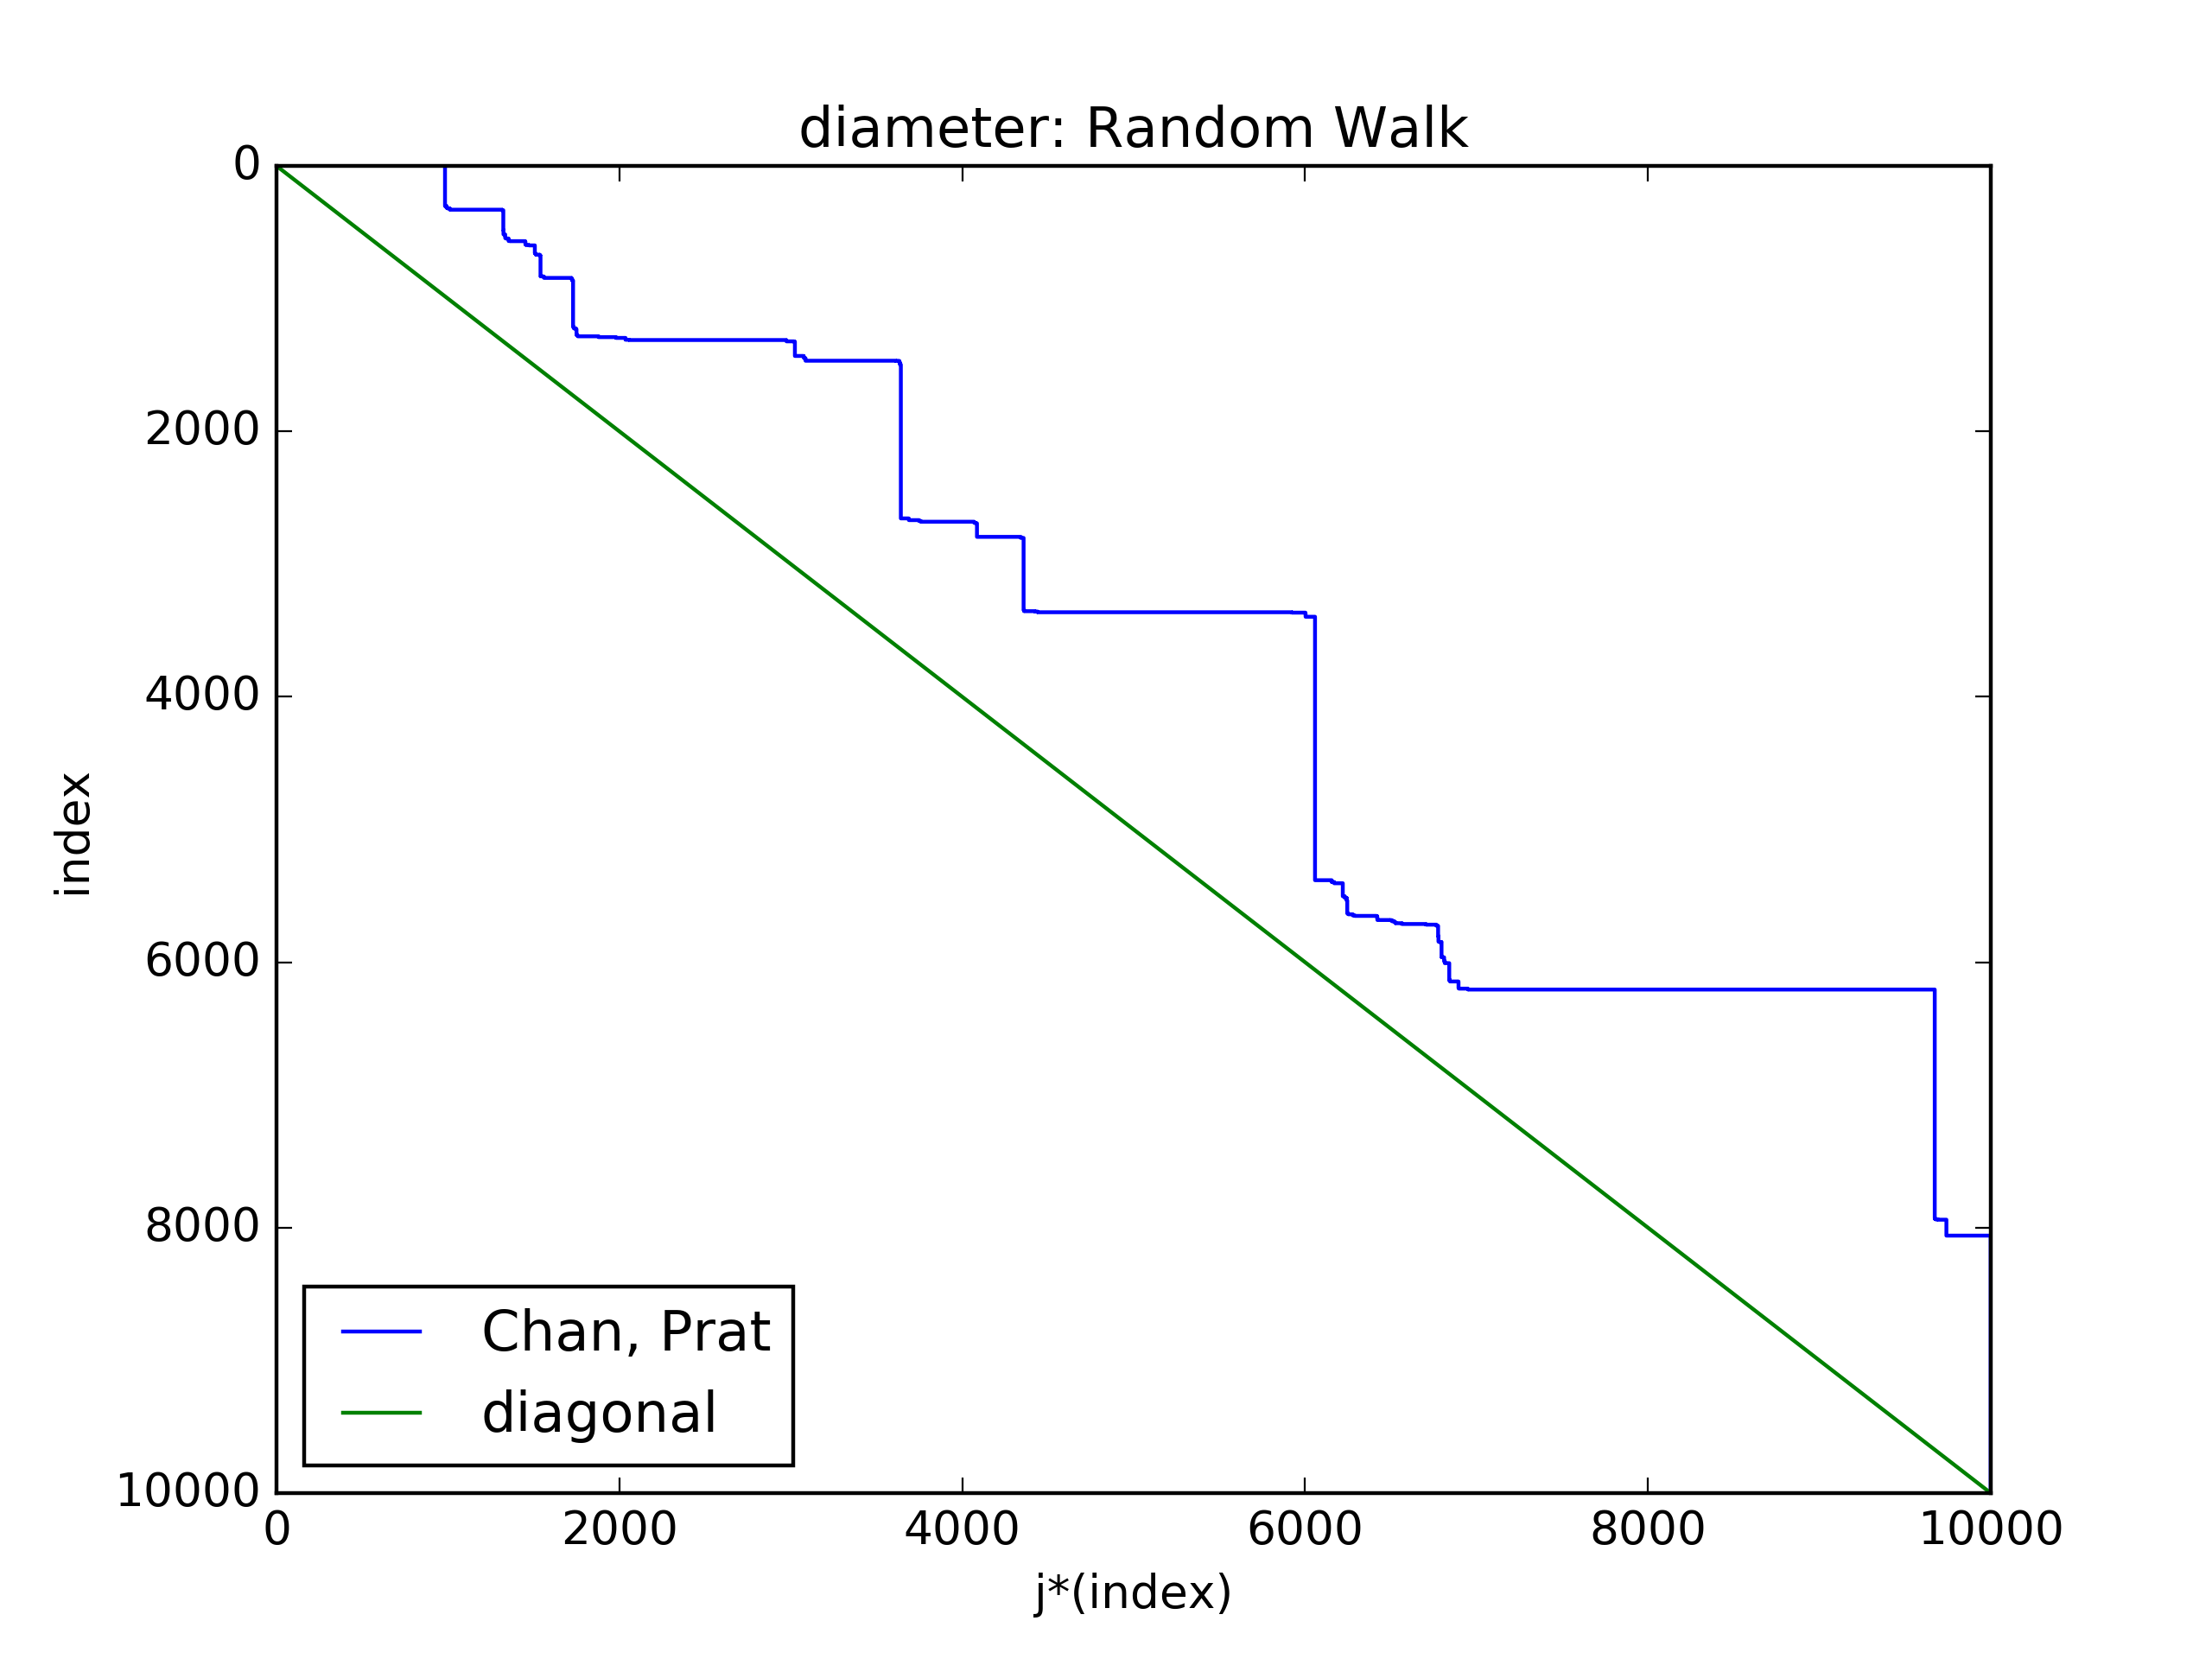
\includegraphics[height=8cm]{../plots/diameter_random_walk}
  \caption{Property matrix for checking 1 distance closeness on a random walk with step size 0.3}
  \label{fig:diameter_demo}
\end{figure}

TODO(arsen): Fix timing comparison 

\begin{figure}[!ht]
  \centering
  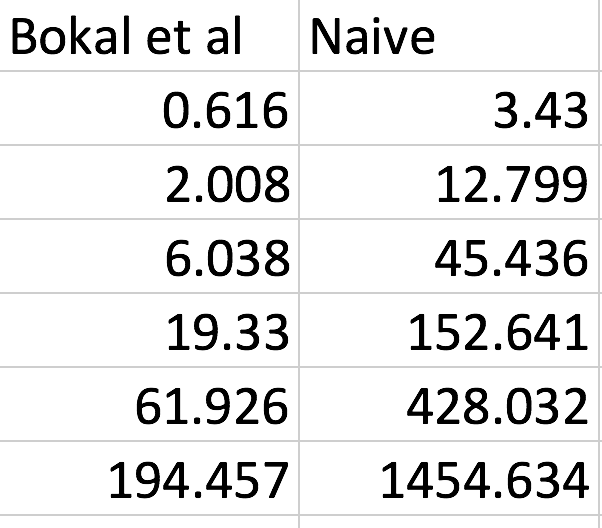
\includegraphics[height=5cm]{figures/diameter_comparison}
  \caption{Runtimes (in millseconds) of Naive and Chan, Prat [Similar to Figure \ref{fig:monotonicity_comparison}}
  \label{fig:diameter_comparison}
\end{figure}

\section{Conclusion}
\label{sec:conclusion}

TODO: Finish Conclusion after other sections are polished.

It was really challanging to do an implementation project in computational geometry, some sentences in the papers take 100+ lines of code to implement. Thus, for small datasets, added complexity is not worth the speedup gained by the algorithm.

This was a great project otherwise, we've implemented couple of algorithms that we have seen during the lecture - sweep line, range tree, intersection of convex polygons using envelopes. Also couple that we had not found in Bokal et al and Chan, Prat.

\bibliographystyle{unsrt}
\bibliography{papers}
\end{document}
